%%%%%%%%%%%%%%%%%%%%%%%%%%%%%%%%%%%%%%%%%%%%%%%%%%%%%%%%%%%%%%%%%%%%%%%%%%%%%%%%
%%
%% Uppsala Beamer theme example by Frédéric Haziza <daz@it.uu.se>
%%
%% Describing beamerthemeUppsala version 2008/05/15
%%
%% If you have more than three sections or more than three subsections in at least
%% one section, you might want to use the [hideallsubsections] or
%% [hideothersubsections] switch.  In this case, only the current (sub-) section is
%% displayed in the sidebar and not the full overview.
%%
%% Options are:
%% ===========
%% * hideallsubsections, hideothersubsections
%% * nonumbers,totalnumber
%% * withnav, mylogo
%% * grey
%% * noprogressbar
%%
%% For the sidebar layout:
%% * subsectionsattop, sectionpathattop
%% 
%% Removed
%% =======
%% * sidebarshades
%%
%% Tip
%% ===
%% latex this file to see the theme in action
%%
%%%%%%%%%%%%%%%%%%%%%%%%%%%%%%%%%%%%%%%%%%%%%%%%%%%%%%%%%%%%%%%%%%%%%%%%%%%%%%%%

\documentclass{beamer}
%\documentclass[handout]{beamer}
%\documentclass[notes]{beamer}
%\documentclass[trans]{beamer}

\usetheme[hideothersubsections]{Uppsala}

\usepackage{hyperref}
\usepackage{pgf}
\usepackage{tikz}
\usepgflibrary{arrows}
\usepgflibrary{shapes}
\usetikzlibrary{%
  arrows,%
  calc,%
  fit,%
  patterns,%
  plotmarks,%
  shapes.geometric,%
  shapes.misc,%
  shapes.symbols,%
  shapes.arrows,%
  shapes.callouts,%
  shapes.multipart,%
  shapes.gates.logic.US,%
  shapes.gates.logic.IEC,%
  er,%
  automata,%
  backgrounds,%
  chains,%
  topaths,%
  trees,%
  petri,%
  mindmap,%
  matrix,%
  calendar,%
  folding,%
  fadings,%
  through,%
  positioning,%
  scopes,%
  decorations.fractals,%
  decorations.shapes,%
  decorations.text,%
  decorations.pathmorphing,%
  decorations.pathreplacing,%
  decorations.footprints,%
  decorations.markings,%
  shadows}

%\usepackage[english]{babel} % or whatever
\usepackage[utf8]{inputenc} % or whatever

\usepackage{mathptmx}
\usepackage{helvet}
%\usepackage{courier}

\usepackage[T1]{fontenc}
% Or whatever. Note that the encoding and the font should match. If T1
% does not look nice, try deleting the line with the fontenc.
\usepackage[makeroom]{cancel}
\usepackage{cwpuzzle}
\usepackage[normalem]{ulem}
\usepackage{multirow,bigdelim}
\usepackage{astra}

\newcommand{\Dom}[1]{\text{dom}({#1})}
\newcommand{\Table}{\Constraint{Table}}

% SparseBitSet
\newcommand{\Words}{\texttt{words}}
\newcommand{\Index}{\texttt{index}}
\newcommand{\Mask}{\texttt{mask}}
\newcommand{\Limit}{\texttt{limit}}
\newcommand{\SparseBitSet}{\texttt{SparseBitSet}}
\newcommand{\Offset}{\localvar{offset}}

% CT Propagator
\newcommand{\Scp}{\texttt{vars}}
\newcommand{\CurrTable}{\texttt{validTuples}}
\newcommand{\Sval}{\texttt{S^{val}}}
\newcommand{\Ssup}{\texttt{S^{sup}}}
\newcommand{\LastSizes}{\texttt{lastSize}}
\newcommand{\Supports}{\texttt{supports}}
\newcommand{\Residues}{\texttt{residues}}

% Pseduo code
\newcommand{\ForEach}[1]{\textbf{foreach } {#1} \textbf{ do }}
\newcommand{\ForEachTo}[3]{\textbf{foreach } {#1} \textbf{ from } {#2} 
  \textbf{ to } {#3} \textbf{ do }}
\newcommand{\ForEachDownTo}[3]{\textbf{foreach } {#1} \textbf{ from } {#2} 
  \textbf{ downto } {#3} \textbf{ do }}
\newcommand{\Break}{\textbf{break~}}
\newcommand{\While}[1]{\textbf{while~} {#1} \textbf{~do~}}

\renewcommand{\algorithmicfor}{\textbf{Method}}
\renewcommand{\algorithmicdo}{}
\renewcommand{\algorithmicforall}{\textbf{foreach}}
%\renewcommand{\algorithmicwhile}{\textbf{foreach}}

\newcommand{\Func}[2]{\FOR{#1(#2)}}
\newcommand{\FuncRet}[3]{\FOR{#1(#2) \ : \ \textbf{#3}}}
\newcommand{\Endfunc}{\ENDFOR}
\newcommand{\To}{~\bf{to}~}
\newcommand{\Downto}{~{\bf{downto}}~}
\newcommand{\For}[3]{\FOR{${#1} \leftarrow {#2} \To {#3}$ \textbf{do}}}
\newcommand{\ForDown}[3]{\FOR{${#1} \leftarrow {#2} \Downto {#3}$ \textbf{do}}}
\newcommand{\FOREACH}[1]{\FORALL{{#1} \textbf{do}}}
\newcommand{\ENDFOREACH}{\ENDFOR}

\renewcommand{\algorithmiccomment}[1]{\hfill // #1}
\def\PROCEDURE{\item[\textbf{PROCEDURE}]}
\def\FAILED{\textbf{FAILED}}
\def\NOFIX{\textbf{NOFIX}}
\def\FIX{\textbf{FIX}}
\def\SUBSUMED{\textbf{SUBSUMED}}
\def\FAIL{\textbf{FAIL}}
\def\bool{\mathit{bool}}
\def\StatusMessage{\mathit{StatusMessage}}
\def\FindSupport{\textsc{FindSupport}}
\def\RemoveSupport{\textsc{RemoveSupport}}
\def\Extensional{\textsc{Extensional}}
\def\CompactTable{\textsc{CompactTable}}
\def\UpdateTable{\textsc{UpdateTable}}
\def\FilterDomains{\textsc{FilterDomains}}
\def\FixDomains{\textsc{FixDomains}}
\def\InitialiseCT{\textsc{InitialiseCT}}
\def\IndexOfFixed{\mathit{index\_of\_fixed}}


\newcommand{\ITE}[3]{\text{\bf ~if~} #1 \text{\bf ~then~} #2 \text{\bf ~else~} #3 \text{\bf ~endif}}

\newcommand{\function}[1]{\mathrm{#1}}
\newcommand{\localvar}[1]{\mathit{#1}}

\newlength\myindent
\setlength\myindent{2em}
\newcommand\bindent{%
  \begingroup
  \setlength{\itemindent}{\myindent}
  \addtolength{\algorithmicindent}{\myindent}
}
\newcommand\eindent{\endgroup}

\newcommand{\INDSTATE}[1][1]{\STATE\hspace{#1\algorithmicindent}}
\newcommand{\INDRETURN}[1][1]{\STATE\hspace{#1\algorithmicindent}\textbf{return~}}
\newcommand{\INDIF}[2][1]{\STATE\hspace{#1\algorithmicindent}
  \textbf{if~}{#2}\textbf{~then}}
\newcommand{\INDELSE}[1][1]{\STATE\hspace{#1\algorithmicindent}\textbf{else~}}
\newcommand{\INDELSEIF}[2][1]{\STATE\hspace{#1\algorithmicindent}
  \textbf{else if~}{#2}\textbf{~then}}

\newcommand{\CTpaper}[0]{DBLP:conf/cp/DemeulenaereHLP16}

\newcommand{\stressed}[1]{\emph{{\color{red!50}{#1}}}}

%% -----------------------------------------------------------
%% MISC. INFORMATION
%% -----------------------------------------------------------

\title{Implementation and Evaluation of a Compact-Table Propagator in Gecode}
%\subtitle{Bachelor's thesis}

\author[Linnea Ingmar | \emph{linnea.ingmar.3244@student.uu.se}] % appears in the footline
{Linnea Ingmar \\ <\texttt{linnea.ingmar.3244@student.uu.se}>}


\institute[Dept. of Information Technology] % appears in the footline
{
  The ASTRA Group\\ on Combinatorial Optimisation \\
  Uppsala University
}


\date[\today] % appears in the bottom of the sidebar
{\today}

%% \logo{...}

%% This is only inserted into the PDF information catalog. Can be left out.
\subject{Unofficial Beamer Theme for Uppsala University}

%% -----------------------------------------------------------
%% Extra ``local'' settings
%% -----------------------------------------------------------

% Comment out this, if you do not want the table of contents to pop up at
% the beginning of each (sub)section:
\AtBeginSection[]
{
  \begin{frame}<beamer> % with <beamer> => doesn't appear in handout mode
    \frametitle{Outline} %% Put the title you want, or none!
    %\tableofcontents[currentsection,currentsubsection]
    \tableofcontents[currentsection]
  \end{frame}
}

%% Unfolds piecewise element with shading.
%% Text appears, shaded, and the audience knows that somehting is coming
%% Note: if you set the number too high, the audience will try to read the 
%% text that now shows up more, and will be disturbed.
%% ``dynamic'' makes elements show gradually more and more.
\setbeamercovered{transparent=5}
%% \setbeamercovered{dynamic=5}

%% -----------------------------------------------------------

\begin{document}

\begin{frame}[plain] %% Gets the frame to fill up the page, no menu/sidebar/footline
  \titlepage
  
  \begin{figure}
    \begin{flushright}
        \begin{tabular}[t,right]{lr}
          Supervisor: & Mats Carlsson (SICS) \\
          Reviewer:   & Pierre Flener
        \end{tabular}
      \end{flushright}
  \end{figure}

\end{frame}

\begin{frame}
    \frametitle{Outline}
    \tableofcontents[currentsection]
\end{frame}

\section{Background}

\subsection{Constraint Programming}
% Kakuro

\begin{frame}
  \frametitle{Kakuro puzzle}
  \begin{minipage}{0.45\textwidth}
    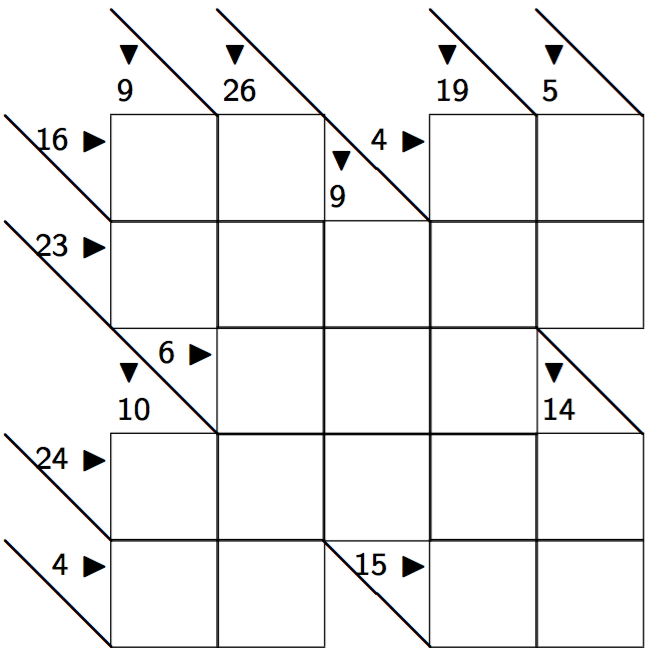
\includegraphics[scale=0.15]{kakuro.png}
  \end{minipage}
  \begin{minipage}{0.45\textwidth}
    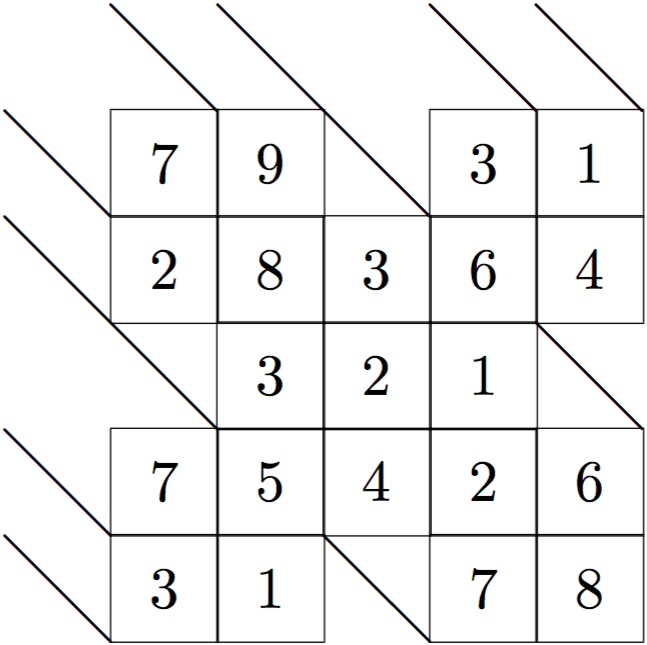
\includegraphics[scale=0.15]{kakuro-sol.png}
  \end{minipage}

  \bigskip

  Assign the cells digits from~$1$ to~$9$ such that for each row and column:
  \begin{itemize}
    \item digits are distinct, and
    \item the sum of the digits is equal to the \emph{clue}
    \end{itemize}

\end{frame}

\begin{frame}
  \frametitle{Kakuro puzzle as a constraint problem (1)}
  \begin{minipage}{0.5\textwidth}
    \begin{description}
      \item[Variables] One per cell.
      \item[Domains] $\Set{1...9}$ for all variables.
      \item[Constraints] For each row and column: \stressed{distinct} digits,
        and the \stressed{sum} of the digits is equal to the clue.
    \end{description} 
  \end{minipage}
  \begin{minipage}{0.45\textwidth}
    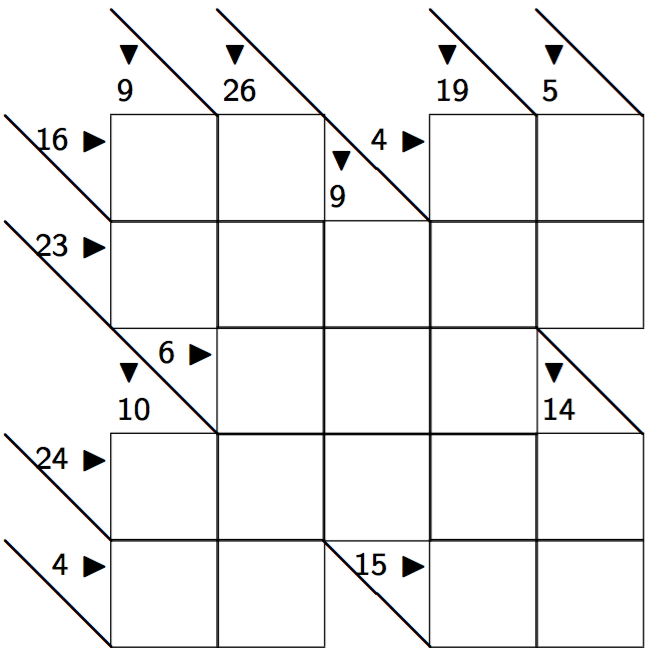
\includegraphics[scale=0.2]{kakuro.png}
  \end{minipage}
\end{frame}

\begin{frame}
  \frametitle{Kakuro puzzle as a constraint problem (2)}
  \begin{minipage}{0.5\textwidth}
    \begin{description}
      \item[Variables] One per cell.
      \item[Domains] $\Set{1...9}$ for all variables.
      \item[Constraints] For each row and column: state the \stressed{possible
        combinations of values} that the variables can take.
    \end{description} 
  \end{minipage}
  \begin{minipage}{0.45\textwidth}
    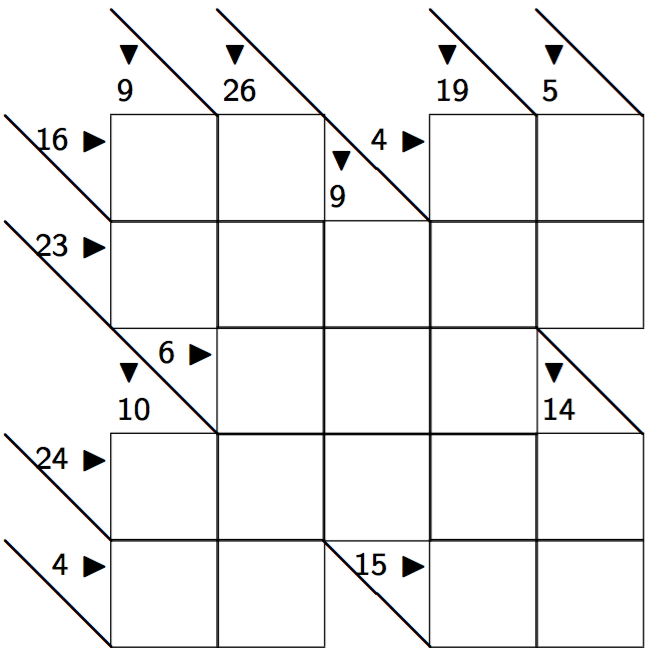
\includegraphics[scale=0.2]{kakuro.png}
  \end{minipage}

  \bigskip
  For an entry of size~$2$ and clue~$4$:~$\Tuple{1,3}$ and~$\Tuple{3,1}$
  are the only combinations.
\end{frame}


% - CSP
\begin{frame}
  \frametitle{Constraint problems (definition)}
  \begin{definition}[Constraint problem]
    A \textbf{constraint satisfaction problem (CSP)} is a 
    triple\\
    \begin{center}
      $\left<V,D,C\right>$\\      
    \end{center}
    where: \\
    \begin{itemize}
      \item $V = v_1, \ldots, v_n$ is a finite sequence of variables,
      \item $D = D_1, \ldots, D_n$ is a finite sequence of domains, that are
        possible values for the respective variable,
      \item $C = \Set{c_1, \ldots, c_m}$ is a finite set of constraints, 
        each on a subset of~$V$. 
        Express relations among the variables that have to be true.
    \end{itemize}
  \end{definition}
\end{frame}

% Define:
% - Constraints?
% \begin{frame}
%   \frametitle{Constraints and \Table~constraints (definitions)}
%   \begin{definition}[Constraint]
%     \label{def:constraint}
%     A \textbf{constraint} on a finite sequene of~$n$ variables~$X$
%     is a relation, denoted~$rel(c)$, that
%     contains the set of allowed~$n$-tuples for~$X$.
%     Each variable~$x_i \in X$ has a corresponding \emph{domain}~$D_i$
%     that is the set of possible values that~$x_i$ can take.
%   \end{definition}
  
%   \begin{definition}[\Table~constraints]
%     A \Table~constraint explicitly lists~$rel(c)$ as a sequence
%     of~$n$-tuples.
%   \end{definition}

%   \begin{example}
%     \begin{tabular}{cc}
%       \Table($\Set{x_0,x_1}, \Set{\Tuple{7,9}, \Tuple/Users/linneaingmar/Documents/Kurser/exjobb/presentation/source.tex{9,7}}$) & \includegraphics[scale=0.2]{kakuro-hint.png}
%     \end{tabular}
%   \end{example}  

% \end{frame}


% - Store

\begin{frame}
  \frametitle{Constraint Propagation}
  \begin{itemize}
    \item Constraint store
    \item Propagator
    \item Constraint propagation
  \end{itemize}
\end{frame}

\begin{frame}
  \frametitle{Constraint Stores}
  \begin{definition}[Constraint store]
    A \textbf{constraint store}~$s$ is a function mapping variables
    to domains:
    \begin{center}
      $s: variables \mapsto domains$
    \end{center}
  \end{definition}

  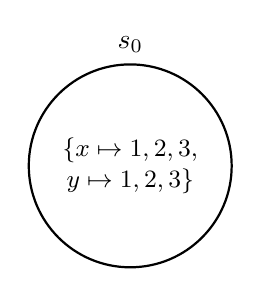
\begin{tikzpicture}[->,>=stealth',auto,node distance=3cm,
    thick,main node/.style={circle,draw,font=\sffamily\Large\bfseries}]
    \node[label={$s_0$},draw,circle](1){
      \small
      \begin{tabular}{c}
        $\{x \mapsto \Set{1,2,3},$\\ 
        $y\mapsto\Set{1,2,3}\}$
      \end{tabular}
    };
    % \node[draw,circle,right of=1,node distance=13em](2){
    %   \small
    %   \begin{tabular}{c}
    %     $\{x \mapsto \Set{1,2},$\\ 
    %     $y\mapsto\Set{1,2,3}\}$
    %   \end{tabular}
    % };
    % \path[every node/.style={font=\sffamily\small}] 
    % (1) edge node [bend right] {$p_{x<y}$} (2);
    
  \end{tikzpicture}
  

    % \begin{minipage}{0.5\textwidth}
    %   $s(x_0) = \Set{1,2,3,4,5,6,7,8,9}$\\
    %   $s(x_1) = \Set{1,2,3,4,5,6,7,8,9}$\\
    %   $\ldots$
    % \end{minipage}
    % \begin{minipage}{0.45\textwidth}
    %   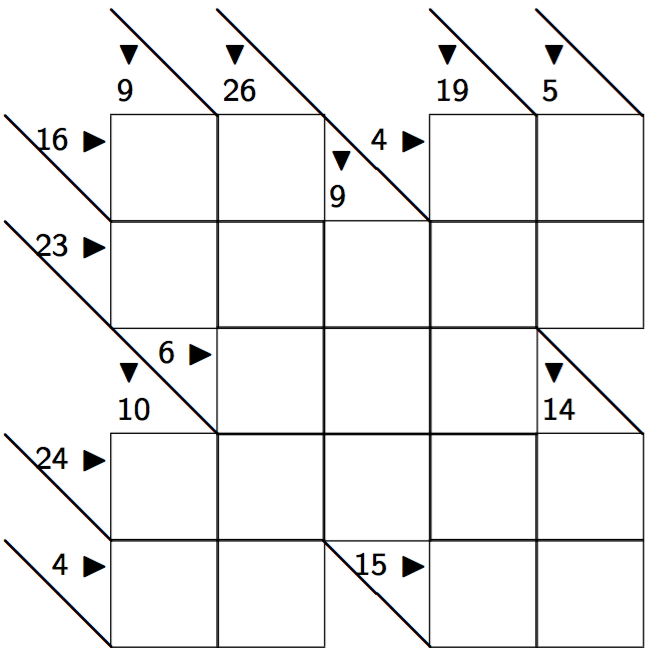
\includegraphics[scale=0.15]{kakuro.png}
    % \end{minipage}
      % We denote the domain of
    % a variable~$v_i$ under~$s$ by~$s(v_i)$ or~$\Dom{v_i}$.
  %Furthermore, a store~$s$...

  % \begin{itemize}
  %   \item ...is a \emph{failed store} iff $s(v_i) = \emptyset$ for some~$v_i \in V$.
  %   \item ...is an \emph{assignment store} iff~$\Cardinality{s(v_i)} = 1$ for all~$v_i \in V$.
  %   \item ...is a \emph{solution store} for a constraint~$c$ iff~$s$ is an assignment store
  %     that constructs a solution to~$c$.
  % \end{itemize}
\end{frame}

\begin{frame}
  \frametitle{Propagators}
  \begin{definition}[Propagator]
    A \textbf{propagator}~$p$ is a function mapping stores to stores:
    \begin{center}
      $p: store \mapsto store$ 
    \end{center}
  \end{definition}

  \begin{itemize}
  \item   Implement constraints
  % \item   Prune values from the domains that are in conflict 
  %   with the constraint
  \end{itemize}

  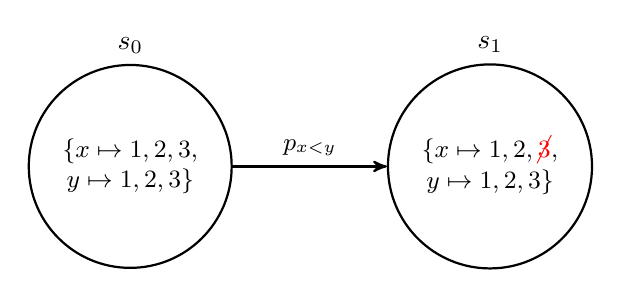
\begin{tikzpicture}[->,>=stealth',auto,node distance=3cm,
  thick,main node/.style={circle,draw,font=\sffamily\Large\bfseries}]
    \node[label=$s_0$,draw,circle](1){
      \small
      \begin{tabular}{c}
        $\{x \mapsto \Set{1,2,3},$\\ 
        $y\mapsto\Set{1,2,3}\}$
      \end{tabular}
    };
    \node[label=$s_1$,draw,circle,right of=1,node distance=13em](2){
      \small
      \begin{tabular}{c}
        $\{x \mapsto \Set{1,2,{\color{red}\cancel{3}}},$\\ 
        $y\mapsto\Set{1,2,3}\}$
      \end{tabular}
    };
    \path[every node/.style={font=\sffamily\small}] 
    (1) edge node [bend right] {$p_{x<y}$} (2);
    
  \end{tikzpicture}

  % \begin{minipage}{0.5\textwidth}
  %   $x_0 \in \Set{1,2,3,4,5,6,7,8,9}$\\
  %   $x_1 \in \Set{1,2,3,4,5,6,7,8,9}$\\
  %   $\ldots$
  %   \Table($\Set{x_0,x_1}, \Set{\Tuple{7,9}, \Tuple{9,7}}$)\\
  %   $\ldots$
  % \end{minipage}
  % \begin{minipage}{0.45\textwidth}
  %   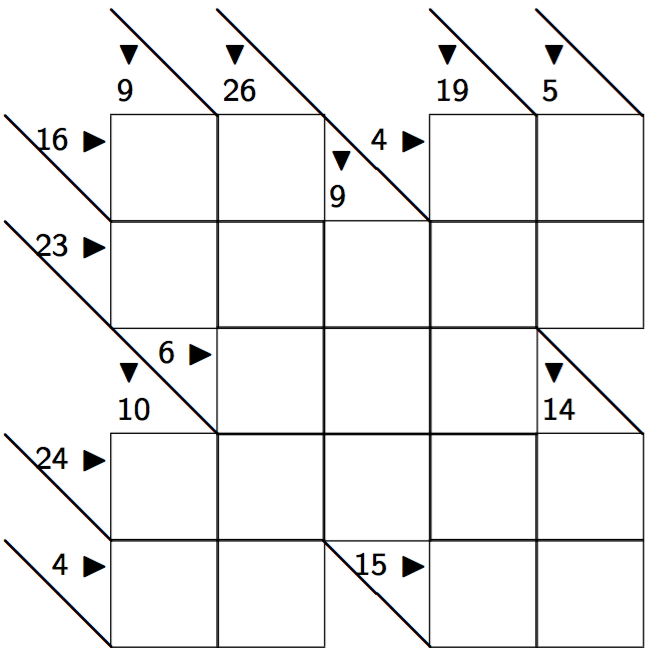
\includegraphics[scale=0.15]{kakuro.png}
  % \end{minipage}

  % Furthermore, a propagator~$p$...
  % \begin{itemize}
  %   \item ...is a decreasing function (i.e. can only remove values and 
  %     not add new values).
  %   \item ...is a monotonic function (not a strict obligation).
  %   \item ...must faithfully implement its constraint.
  %   \item ...signals a \emph{status message}.
  % \end{itemize}
\end{frame}

\begin{frame}
  \frametitle{Constraint Propagation}
  %Prune values from the variables that  
  \begin{minipage}{0.5\textwidth}
    \only<1>{$x_0 \in \Set{1,2,3,4,5,6,7,8,9}$}
    \only<2>{$x_0 \in \Set{\cancel{1},\cancel{2},\cancel{3},\cancel{4},\cancel{5},\cancel{6},7,\cancel{8},9}$}
    \only<3->{$x_0 \in \Set{\cancel{1},\cancel{2},\cancel{3},\cancel{4},\cancel{5},\cancel{6},\textbf{7},\cancel{8},\cancel{9}}$} \\
    \only<1>{$x_1 \in \Set{1,2,3,4,5,6,7,8,9}$}
    \only<2-3>{$x_1 \in \Set{\cancel{1},\cancel{2},\cancel{3},\cancel{4},\cancel{5},\cancel{6},7,\cancel{8},9}$}
    \only<4->{$x_1 \in \Set{\cancel{1},\cancel{2},\cancel{3},\cancel{4},\cancel{5},\cancel{6},\cancel{7},\cancel{8},\textbf{9}}$}\\
    $\ldots$ \\
    \only<1-2>{$x_4 \in \Set{1,2,3,4,5,6,7,8,9}$}
    \only<3->{$x_4 \in \Set{\cancel{1},\textbf{2},\cancel{3},\cancel{4},\cancel{5},\cancel{6},\cancel{7},\cancel{8},\cancel{9}}$}\\
    $\ldots$
    %$\Table(\Set{x_0,x_1},\Set{\Tuple{7,9},\Tuple{9,7}})$
    
    \begin{tabular}{ccc}
      
      \begin{tabular}{cc}
        $x_0$ & $x_1$ \\
        \hline
        $7$   & $9$ \\
        \only<1-3>{$9$   & $7$ \\} 
        \only<4->{\sout{$9$}   & \sout{$7$} \\} 
      \end{tabular} & 
                         \only<1>{
                          \begin{tabular}{cc}
                            $x_0$ & $x_4$ \\
                            \hline
                            $1$   & $8$ \\
                            $2$   & $7$ \\
                            $3$   & $6$ \\
                            $4$   & $5$ \\
                            $5$   & $4$ \\
                            $6$   & $3$ \\
                            $7$   & $2$ \\
                            $8$   & $1$ \\
                          \end{tabular} & $\ldots$}
                          \only<2->{
                          \begin{tabular}{cc}
                            $x_0$ & $x_4$ \\
                            \hline
                            \sout{$1$}   & \sout{$8$} \\
                            \sout{$2$}   & \sout{$7$} \\
                            \sout{$3$}   & \sout{$6$} \\
                            \sout{$4$}   & \sout{$5$} \\
                            \sout{$5$}   & \sout{$4$} \\
                            \sout{$6$}   & \sout{$3$} \\
                            $7$   & $2$ \\
                            \sout{$8$}  &  \sout{$1$}\\
                          \end{tabular} & $\ldots$}

    \end{tabular}

  \end{minipage}
  \begin{minipage}{0.45\textwidth}
    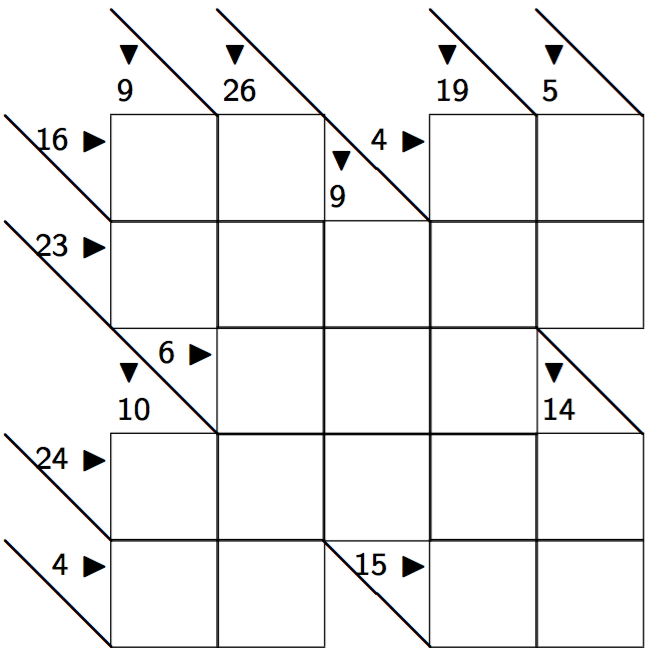
\includegraphics[scale=0.2]{kakuro.png}
  \end{minipage}
\end{frame}

\begin{frame}
  \frametitle{\Table~constraints}
  \begin{definition}[\Table~constraint]
    A \Table~constraint lists the possible combinations of values
    that the variables can take as a sequence of~$n$-tuples.
  \end{definition}

  \bigskip
  \bigskip

  \begin{tabular}{cr}
      \Table($\Set{x_0,x_1}$, $[\Tuple{7,9},\Tuple{9,7}]$)\\
    \bigskip
    \begin{tabular}{cc}
      $x_0$ & $x_1$ \\
      \hline
      $7$   & $9$ \\
      $9$   & $7$ \\
    \end{tabular} &
                    \includegraphics[scale=0.3]{kakuro-hint.png}
    
  \end{tabular}
\end{frame}

\subsection{Gecode}

\begin{frame}
  \frametitle{Gecode}
  \textbf{Gecode} (Generic Constraint Development Environment)
  is...

  \begin{itemize}
    \item ...a constraint solver (a software that solves constraint problems).
    \item ...written in C++, modular, extensible, and has state-of-the-art performance.
    \item ...supports the programming of new propagators.
  \end{itemize}

  Two existing propagators for the~\Table~constraint
  % , and one for the 
  % related constraint~\Constraint{Regular}.

\end{frame}

\subsection{The Compact-Table algorithm}

\begin{frame}
  \frametitle{Compact Table}
  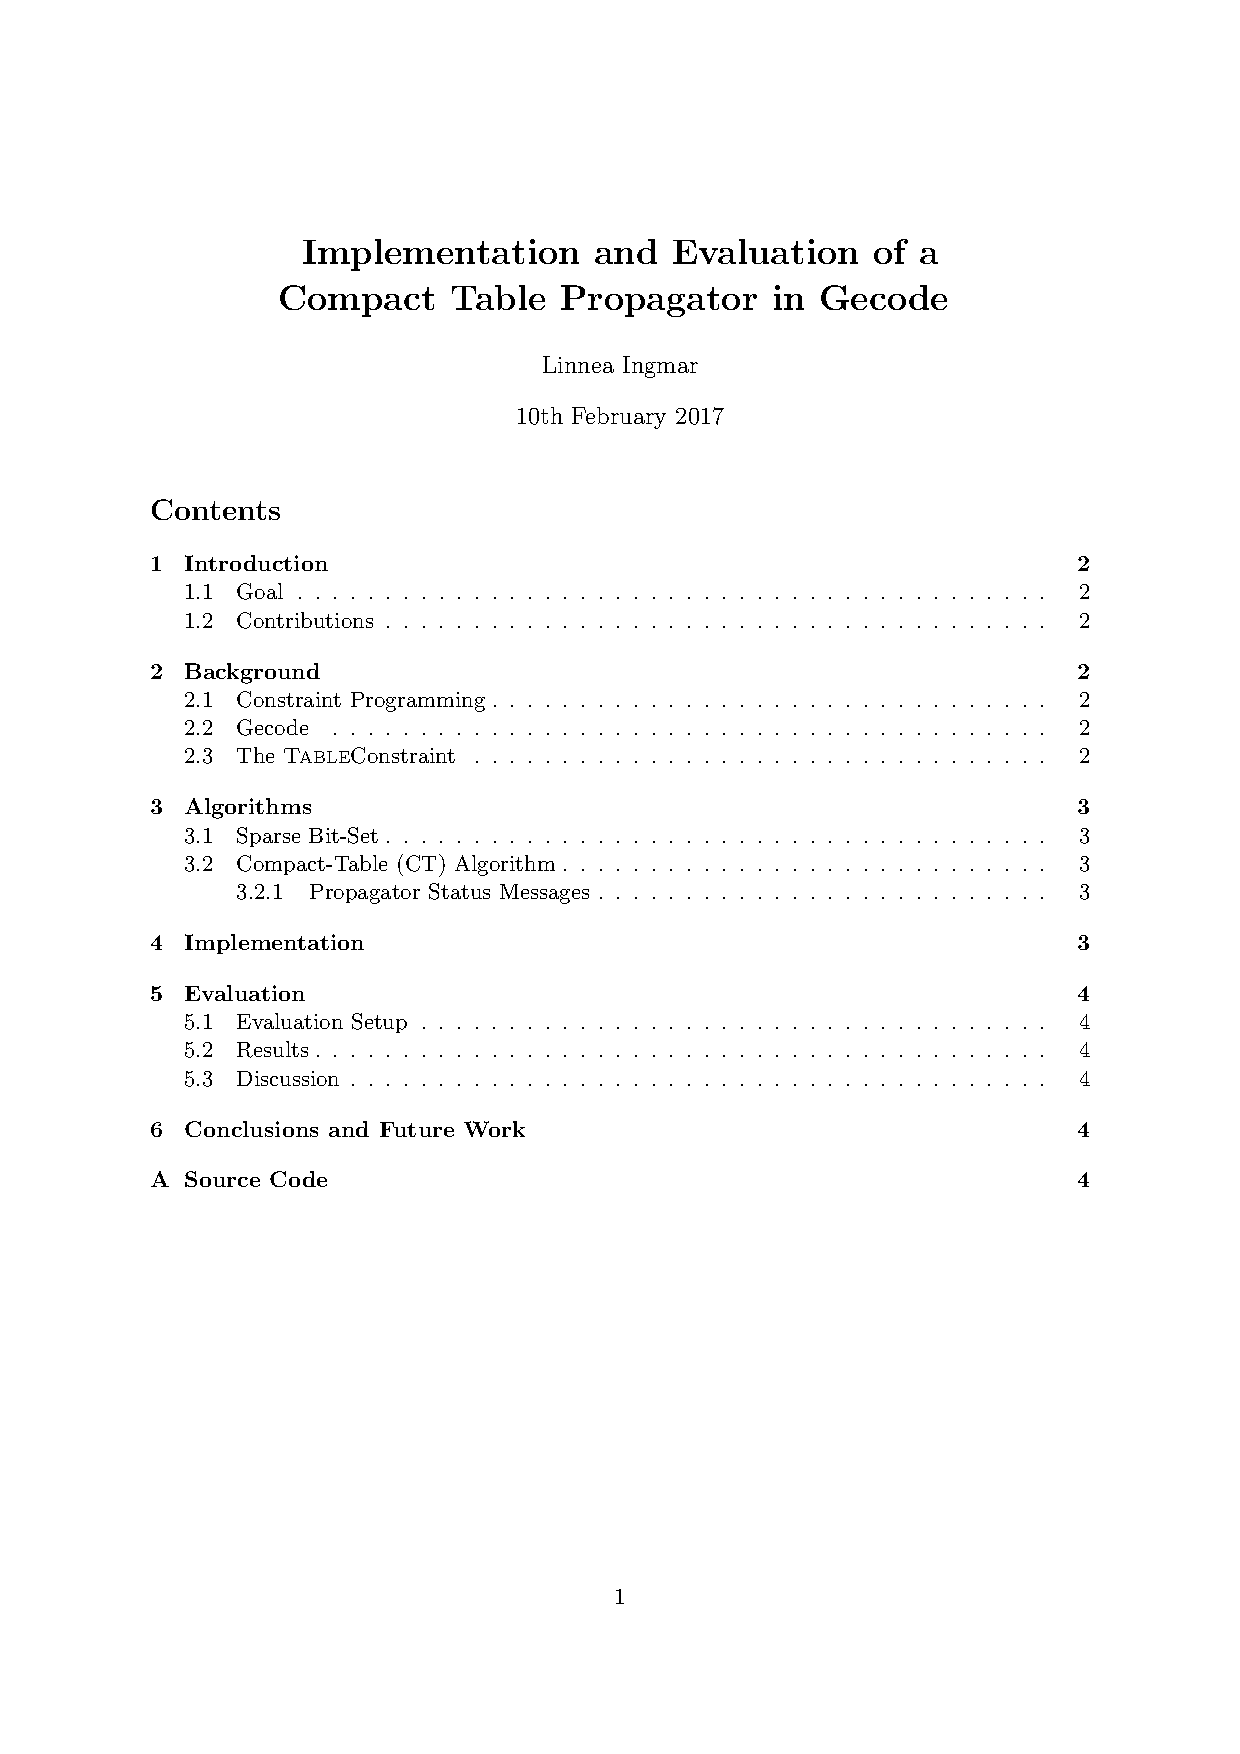
\includegraphics[scale=0.45]{compact-table.png}
\end{frame}

\begin{frame}
  \frametitle{Compact-Table}
  % Efficient
  \begin{itemize}
  \item   A new propagation algorithm for the~\Table~constraint.
  \item   Published in a 2016 paper%~\cite{\CTpaper}.
  \item   No attempt to implement it in Gecode (until now).
  \end{itemize}

\end{frame}

\section{The Compact-Table Algorithm}

\begin{frame}
  \frametitle{The Compact-Table Algorithm}
  \begin{itemize}
  \item \textbf{Initialisation}
  \item \color{gray}Variable modifications
  \item Filtering
   \item {\color{gray}Putting it all together}
  \end{itemize}

\end{frame}

\begin{frame}
  \frametitle{The Compact-Table Algorithm}
  \framesubtitle{Initialisation}
  \small
  \only<1-5>{
    $\Dom{x_0} = \Dom{x_1} = \Dom{x_2} = \Set{1,2,3,4}$
  }
  \only<6->{
    $\Dom{x_0} = \Set{1,2,{\color{red}\cancel{3}},4}$\\
    $\Dom{x_1} = \Dom{x_2} = \Set{1,2,3,4}$
  }

  \bigskip

  \begin{tabular}{l}

    \only<4->{
    %\CurrTable: bit-set with valid tuples\\
    %\phantom{foo}\\
    \small
    \begin{tabular}{cc}
      %\phantom{\texttt{words}}
      \phantom{$\Tuple{x_0,2}$}
      &
        \begin{tabular}{|cccccccc|c}
          \cline{1-8}
          {\textbf{1}} & {\textbf{1}} & {\textbf{1}} & {\textbf{1}} & {\textbf{1}}& {\textbf{1}}& {\textbf{1}} & {\textbf{1}} & \rdelim\}{1}{3mm}[\CurrTable] \\
          \cline{1-8}
        \end{tabular}
    \end{tabular}

    \bigskip
    }
    \\
    \only<5->{
    %\Supports: \\
    %\phantom{foo}\\
    \begin{tabular}{ccc}
      $\Tuple{x_0,1}$
      & 
        \begin{tabular}{|cccccccc|}
          \hline
          0 & \textbf{1} & 0 & 0 & \textbf{1} & 0 & 0 & 0 \\
        \end{tabular}
      &
        \rdelim\}{5}{3mm}[\texttt{supports}]
      \\
      $\Tuple{x_0,2}$
      & 
        \begin{tabular}{|cccccccc|}
          \textbf{1} & 0 & \textbf{1} & 0 & 0 & \textbf{1} & \textbf{1} & 0 \\
        \end{tabular}
      \\
      $\Tuple{x_0,3}$
      & 
        \begin{tabular}{|cccccccc|}
          \alt<6->{{\color{red}0} & \color{red}0 & \color{red}0 & \color{red}0 & \color{red}0 & \color{red}0 & \color{red}0 & {\color{red}0}} 
              {0 & 0 & 0 & 0 & 0 & 0 & 0 & 0} \\
          
        \end{tabular}
      \\
      $\ldots$
      \\
      $\Tuple{x_2,4}$
      & 
        \begin{tabular}{|cccccccc|}
          \textbf{1} & 0 & 0 & 0 & 0 & 0 & 0 & 0 \\
          \hline
        \end{tabular}
      \\
    \end{tabular}
        
    \bigskip
    } 
    \\
    \only<1>{
    \small
        \begin{tabular}{|c|cccccccccccccccc|}
          \hline
          $x_0$ & 1 & 2 & 1 & 2 & 6 & 7 & 4 & 1 & 7 & 8 & 2 & 0 & 2 & 5 & 4 \\
          $x_1$ & 5 & 1& 3 & 4 & 5 & 7 & 2 & 1 & 8 & 9 & 2 & 0 & 3 & 8 & 3 \\
          $x_2$ & 8 & 4& 2 & 2 & 9 & 8 & 1 & 1 & 9 & 6 & 3 & 0 & 1 & 5 & 1 \\
          \hline
        \end{tabular}}
    \only<2>{
    \small
    \begin{tabular}{|c|ccccccccccccccc|}
      \hline
      $x_0$ & 1 & \textbf{2} & \textbf{1} & \textbf{2} & 6 & 7 & \textbf{4} & \textbf{1} & 7 & 8 & \textbf{2} & 0 & \textbf{2} & 5 & \textbf{4} \\
      $x_1$ & 5 & \textbf{1}& \textbf{3} & \textbf{4} & 5 & 7 & \textbf{2} & \textbf{1} & 8 & 9 & \textbf{2} & 0 & \textbf{3} & 8 & \textbf{3} \\
      $x_2$ & 8 & \textbf{4}& \textbf{2} & \textbf{2} & 9 & 8 & \textbf{1} & \textbf{1} & 9 & 6 & \textbf{3} & 0 & \textbf{1} & 5 & \textbf{1} \\
      \hline
    \end{tabular}
    }
    
    \small
    \begin{tabular}{cc}
      &
        \only<3->{
        \begin{tabular}{|c|cccccccc|}
          \hline
          $x_0$ & \textbf{2}& \textbf{1} & \textbf{2} & \textbf{4} & \textbf{1} & \textbf{2} & \textbf{2} & \textbf{4} \\
          $x_1$ & \textbf{1}& \textbf{3} & \textbf{4} & \textbf{2} & \textbf{1} & \textbf{2} & \textbf{3} & \textbf{3} \\
          $x_2$ & \textbf{4}& \textbf{2} & \textbf{2} & \textbf{1} & \textbf{1} & \textbf{3} & \textbf{1} & \textbf{1} \\
          \hline
        \end{tabular}
      }

    \end{tabular}

    \end{tabular}

\end{frame}


\begin{frame}
  \frametitle{The Compact-Table Algorithm}
  \begin{itemize}
  \item {\color{gray}Initialisation}
  \item \textbf{Variable modifications}
  \item {\color{gray}Filtering}
  \item {\color{gray}Putting it all together}
  \end{itemize}
\end{frame}

\begin{frame}
  \frametitle{The Compact-Table Algorithm}
  \framesubtitle{When a variable is modified}
  \only<2->{
    \begin{tabular}{c}
      \small
      \begin{tabular}{ccc}
        \texttt{words} 
        & 
          \begin{tabular}{|cccccccc|}
            \hline
            \alt<7->{{\color{red}0} & {\textbf{1}} & {\textbf{1}} & {\color{red}0} & {\color{red}0}& {\color{red}0}& {\textbf{1}} & {\textbf{1}}}
            {{\textbf{1}} & {\textbf{1}} & {\textbf{1}} & {\textbf{1}} & {\textbf{1}}& {\textbf{1}}& {\textbf{1}} & {\textbf{1}}} \\
            \hline
          \end{tabular}
        &
          \rdelim\}{2}{1mm}[\tiny \CurrTable]
        \\
        \texttt{mask} 
        &
          \begin{tabular}{|cccccccc|}
            \hline
            \alt<5->{{0} & {\textbf{1}} & {\textbf{1}} & {0} & {0}& {0}& {\textbf{1}} & {\textbf{1}}}
            {{0} & {0} & {0} & {0} & {0}& {0}& {0} & {0}} \\
            \hline
          \end{tabular} 
        \\
        \only<3->{
        \phantom{foo} \\
        $\Supports[x_1,3]$ 
        & 
          \begin{tabular}{|cccccccc|}
            \hline
            0 & \textbf{1} & 0 & 0 & 0 & 0 & \textbf{1} & \textbf{1} \\
            \hline
          \end{tabular}
        \\
        $\Supports[x_1,4]$
        & 
          \begin{tabular}{|cccccccc|}
            \hline
            0 & 0 & \textbf{1} & 0 & 0 & 0 & 0 & 0 \\
            \hline
          \end{tabular}
        \\
        }
        \only<8->{
        \phantom{foo} \\
        $x_0$
        &
          \small
          \begin{tabular}{|cccccccc|}
            \hline
            \textbf{\color{red}2}& \textbf{1} & \textbf{2} & \textbf{\color{red}4} & \textbf{\color{red}1} & \textbf{\color{red}2} & \textbf{2} & \textbf{4} \\
          \end{tabular}
        \\
        $x_1$
        &
          \small
          \begin{tabular}{|cccccccc|}
            \textbf{\color{red}1}& \textbf{3} & \textbf{4} & \textbf{\color{red}2} & \textbf{\color{red}1} & \textbf{\color{red}2} & \textbf{3} & \textbf{3} \\
          \end{tabular}
        \\
        $x_2$
        &
          \small
          \begin{tabular}{|cccccccc|}
            \textbf{\color{red}4}& \textbf{2} & \textbf{2} & \textbf{\color{red}1} & \textbf{\color{red}1} & \textbf{\color{red}3} & \textbf{1} & \textbf{1} \\
            \hline
          \end{tabular}
        \\
        }
      \end{tabular}
      \\
      \only<4>{
      \phantom{foo}\\
      \texttt{mask} = \Supports[$x_1,3$] | \Supports[$x_1,4$]\\
      }
      \only<6>{
        \phantom{foo}\\
      \small
      \texttt{words} = \texttt{words} \& \texttt{mask} \\
      }
    \end{tabular}
    \\
  }
  
  \bigskip

  $\Dom{x_0} = \Set{1,2,4}$\\
  $\Dom{x_1} = \Set{\cancel{1},\cancel{2},3,4}$\\
  $\Dom{x_2} = \Set{1,2,3,4}$

\end{frame}

\begin{frame}
  \frametitle{The Compact-Table Algorithm}
  \framesubtitle{When a variable is modified}
  \begin{algorithm}[H]
    \small
    \begin{algorithmic}[1]
        \PROCEDURE \UpdateTable($s$: store, $x$: variable) \label{line:updateTableDelta:1} 
        \STATE $\CurrTable$.clearMask() \label{line:updateTableDelta:4} 
          \FOREACH{$a \in s(x)$} \label{line:updateTableDelta:8} 
            \STATE $\CurrTable$.addToMask($\Supports[x,a]$) \label{line:updateTableDelta:9} 
          \ENDFOREACH      
        \STATE $\CurrTable$.intersectWithMask() \label{line:updateTable:10} 
    \end{algorithmic}
  \end{algorithm}
\end{frame}

\begin{frame}
  \frametitle{The Compact-Table Algorithm}
  \begin{itemize}
  \item {\color{gray}Initialisation}
  \item {\color{gray}Variable modifications}
  \item \textbf{Filtering}
  \item {\color{gray}Putting it all together}
  \end{itemize}
\end{frame}

\begin{frame}
  \frametitle{Compact-Table Algorithm}
  \framesubtitle{Filtering}
    
  \begin{itemize}
    \item Intersect every support entry with~$\CurrTable$
    \item Remove value if intersection is empty
  \end{itemize}
  
  \bigskip

  \begin{tabular}{c}
      \CurrTable:\\
      \small
      \begin{tabular}{cc}
        \texttt{words} 
        & 
          \begin{tabular}{|cccccccc|}
            \hline
            {0} & {\textbf{1}} & {\textbf{1}} & {0} & {0} & {0} & {\textbf{1}} & {\textbf{1}} \\
            \hline
          \end{tabular}
      \end{tabular} \\
    \\
    \& \\
    \phantom{foo}
    \\
    \small
    \begin{tabular}{cc}
      $\Tuple{x_2,1}$
        & 
          \begin{tabular}{|cccccccc|}
            \hline
            \alt<2->{\color{green}0 & \color{green}0 & \color{green}0 & \color{green}\textbf{1} & \color{green}\textbf{1} & \color{green}0 & \color{green}\textbf{1} & \color{green}\textbf{1}}
            {0 & 0 & 0 & \textbf{1} & \textbf{1} & 0 & \textbf{1} & \textbf{1}} \\
          \end{tabular}
        \\
        $\Tuple{x_2,2}$
        & 
          \begin{tabular}{|cccccccc|}
            \alt<3->
            {\color{green}0 & \color{green}\textbf{1} & \color{green}\textbf{1} & \color{green}0 & \color{green}0 & \color{green}0 & \color{green}0 & \color{green}0}
            {0 & \textbf{1} & \textbf{1} & 0 & 0 & 0 & 0 & 0} \\
          \end{tabular}
        \\
        $\Tuple{x_2,3}$
        & 
          \begin{tabular}{|cccccccc|}
            \alt<4->
            {\color{red}0 & \color{red}0 & \color{red}0 & \color{red}0 & \color{red}0 & \color{red}\textbf{1} & \color{red}0 & \color{red}0}
            {0 & 0 & 0 & 0 & 0 & \textbf{1} & 0 & 0} \\
          \end{tabular}
        \\
        $\Tuple{x_2,4}$
        & 
          \begin{tabular}{|cccccccc|}
            \alt<5->
            {\color{red}\textbf{1} & \color{red}0 & \color{red}0 & \color{red}0 & \color{red}0 & \color{red}0 & \color{red}0 & \color{red}0} 
            {\textbf{1} & 0 & 0 & 0 & 0 & 0 & 0 & 0} \\
            \hline
          \end{tabular}
      \\
      \end{tabular}
    \\
    \phantom{foo} \\
    \alt<6>    
    {$\Dom{x_2} = \Set{1,2,{\color{red}\cancel{3}},{\color{red}\cancel{4}}}$}
    {$\Dom{x_2} = \Set{1,2,3,4}$}
    \end{tabular}
    
\end{frame}

\begin{frame}
  \frametitle{Compact-Table Algorithm}
  \framesubtitle{Filtering out values}
  \begin{algorithm}[H]
    \small
    \begin{algorithmic}[1]
      \PROCEDURE \FilterDomains($s$) : store
      \FOREACH{$x \in s \text{~such that~} |s(x)| > 1$}
            \FOREACH{$a \in s(x)$}
              \STATE $\localvar{inde x} \leftarrow \Residues[x,a]$ \COMMENT{remembered last index}
              \IF{$\CurrTable[index] \ \& \ \Supports[x,a][index] = 0$}
                  \STATE $\localvar{index} \leftarrow \CurrTable$.intersectIndex($\Supports[x,a]$)
                  \IF{$\localvar{index~} \neq -1$}
                        \STATE $\Residues[x,a] \leftarrow \localvar{index}$
                  \ELSE
                        \STATE $s \leftarrow s[x \mapsto s(x) \setminus \Set{a}]$
                  \ENDIF
              \ENDIF
             \ENDFOREACH
      \ENDFOREACH
      \RETURN{$s$}
    \end{algorithmic}
  \end{algorithm}
\end{frame}

\begin{frame}
  \frametitle{The Compact-Table Algorithm}
  \begin{itemize}
  \item {\color{gray}Initialisation}
  \item {\color{gray}Variable modifications}
   \item  {\color{gray}Filtering}
  \item \textbf{Putting it all together}
  \end{itemize}
\end{frame}

\begin{frame}
  \frametitle{The Compact-Table Algorithm}
  \framesubtitle{Putting it all together}
  \begin{algorithm}[H]
    \small
    \begin{algorithmic}[1]
      \PROCEDURE $\CompactTable(s:\text{store}):\Tuple{StatusMsg,\text{store}}$
      \IF{the propagator is being posted}
        \STATE $s \gets \InitialiseCT(s,T_0)$
        \IF{$s = \emptyset$}
          \RETURN $\Tuple{\FAIL, \emptyset}$
        \ENDIF
      \ELSE
      \FOREACH{variable~$x \in s$ whose domain has changed since last time}
      \STATE \UpdateTable($s,x$)
      \IF{$\CurrTable$.isEmpty()}
      \RETURN $\Tuple{\FAIL,\emptyset}$
      \ENDIF
      \ENDFOREACH
            \IF{\CurrTable~has changed since last time}
            \STATE $s \gets \FilterDomains(s)$
            \ENDIF
      \ENDIF
      \IF{there is at most one unassigned variable left}
      \RETURN $\Tuple{\SUBSUMED, s}$
      \ELSE 
      \RETURN $\Tuple{\FIX,s}$
      \ENDIF
    \end{algorithmic}
  \end{algorithm}
\end{frame}



\section{Evaluation}
\subsection{Setup}
\subsection{Results}
\subsection{Discussion}

\section{Conclusions}


% \section{Introduction}

% \begin{frame}
%   \frametitle{Why}

%   Why use \LaTeX, when there are specialized presentations tools (OpenOffice.org Impress, Keynote, PowerPoint) available?

%   \begin{itemize}
%     \item{Look: The layout of mathematical formulas and program text is much nicer\ldots not to speak from ligatures in ``ordinary'' text}
%     \item{Reuse of material: Going from a paper to a presentation is easy -- just use the same ``codebase''}
%     \item{Portable solution: You can use whichever operating system you like}
%     \item{Durable solution: usually even very old \LaTeX code can be typeset with modern installations}
%   \end{itemize}

% \end{frame}

% \section{Cool Stuff}

% \begin{frame}
%   \frametitle{Mathematics}

%   \begin{example}
%     \begin{equation}
%       \mathit{Hamming} (X,Y) = \sum_{i=1}^{n} f (x_{i}, y_{i})
%     \end{equation}
%   \end{example}

% with $f(x,y)$ defined as follows:

%   \begin{definition}
%     \begin{equation}
%       f(x,y)= \left\{ \begin{array}{ll}
%           0 & \mbox{iff $|x-y| \leq \epsilon_{h}$,} \\
%           1 & \mbox{else.}      \\
%         \end{array}
%       \right.
%     \end{equation}
%   \end{definition}

% \end{frame}

% \begin{frame}
%   \frametitle{Piecewise Text Modification}

%   \onslide<1>
%     Shown on first slide.
%   \onslide<2>
%     Shown on second slide.
%   \onslide<1>
%     Shown on first slide.
%     \begin{itemize}
%   \onslide<2-3>
%         \item Shown on the second and the third slide.
%   \onslide+<3->
%         \item Shown from slide 3 on.
%     \end{itemize}
%     Shown from slide 3 on.
%   \onslide
%     Shown on all slides.

%     \vskip 1cm
%   \onslide<4>
%     \alert<4>{You get fine-grain control over which elements are visible at each time.}

% \end{frame}

% \begin{frame}
%   \frametitle{Using Ti\textit{k}Z for Drawings}

%   % Taken from the PGF Manual
%     \begin{tikzpicture}[scale=0.9]
%       \draw[fill=yellow] (0,0) -- (60:.75cm) arc (60:180:.75cm);
%       \draw(120:0.4cm) node {$\alpha$};
%       \draw[fill=green!30] (0,0) -- (right:.75cm) arc (0:60:.75cm);
%       \draw(30:0.5cm) node {$\beta$};
%       \begin{scope}[shift={(60:2cm)}]
%         \draw[fill=green!30] (0,0) -- (180:.75cm) arc (180:240:.75cm);
%         \draw (30:-0.5cm) node {$\gamma$};
%         \draw[fill=yellow] (0,0) -- (240:.75cm) arc (240:360:.75cm);
%         \draw (-60:0.4cm) node {$\delta$};
%       \end{scope}
%       \begin{scope}[thick]
%         \draw (60:-1cm) node[fill=red!20] {$E$} -- (60:3cm) node[fill=red!20] {$F$};
%         \draw[red] (-2,0) node[left] {$A$} -- (3,0) node[right]{$B$};
%         \draw[blue,shift={(60:2cm)}] (-3,0) node[left] {$C$} -- (2,0) node[right]{$D$};
%       \end{scope}
%       \path (5,-0.5) node (x) {Hello World!}
%       (7.5,2) node[circle,draw](y) {$\int_1^2 x \mathrm d x$};
%       \draw[->,blue] (x) -- (y);
%       \draw[->,red] (x) -| node[near start,below] {\footnotesize Red} (y);
%       \draw[->,orange] (x) .. controls +(up:1cm) and +(left:1cm) .. node[above,sloped] {\footnotesize Orange} (y);
%     \end{tikzpicture}

% \end{frame}

% \note{
%   Example from J\"{o}rg Cassens, University of Trondheim, in his example:
%   \vskip 1cm
%   See \href{http://story.idi.ntnu.no/~cassens/blog/categories/20-LaTeX}{his blog on the Trondheim theme}.
% }

% \begin{frame}
%   \frametitle{Using Ti\textit{k}Z for Petri-Net}
%   \begin{center}
% \begin{tikzpicture}
%   [node distance=1.3cm,>=stealth',bend angle=45,auto,
%    place/.style={circle,thick,draw=blue!75,fill=blue!20,minimum size=6mm},
%    red place/.style={place,draw=red!75,fill=red!20},
%    transition/.style={rectangle,thick,draw=black!75,fill=black!20,minimum size=4mm},
%    every label/.style={red},on grid]

%   \begin{scope}
%     % First net
%     \node [place,tokens=1] (w1)                                    {};
%     \node [place] (c1) [below=of w1]                      {};
%     \node [place] (s)  [below=of c1,label=above:$s\le 3$] {};
%     \node [place] (c2) [below=of s]                       {};
%     \node [place,tokens=1] (w2) [below=of c2]                      {};
    
%     \node [transition] (e1) [left=of c1] {}
%       edge [pre,bend left]                  (w1)
%       edge [post,bend right]                (s)
%       edge [post]                           (c1);

%     \node [transition] (e2) [left=of c2] {}
%       edge [pre,bend right]                 (w2)
%       edge [post,bend left]                 (s)
%       edge [post]                           (c2);
      
%     \node [transition] (l1) [right=of c1] {}
%       edge [pre]                            (c1)
%       edge [pre,bend left]                  (s)
%       edge [post,bend right] node[swap] {2} (w1);

%     \node [transition] (l2) [right=of c2] {}
%       edge [pre]                            (c2)
%       edge [pre,bend right]                 (s)
%       edge [post,bend left]  node {2}       (w2);
%   \end{scope}
  
%   \begin{scope}[xshift=6cm]
%     % Second net
%     \node [place,tokens=1]
%                       (w1')                                                {};
%     \node [place]     (c1') [below=of w1']                                 {};
%     \node [red place] (s1') [below=of c1',xshift=-5mm,label=left:$s$]      {};
%     \node [red place,tokens=3]
%                       (s2') [below=of c1',xshift=5mm,label=right:$\bar s$] {};
%     \node [place]     (c2') [below=of s1',xshift=5mm]                      {};
%     \node [place,tokens=1]
%                       (w2') [below=of c2']                                 {};
    
%     \node [transition] (e1') [left=of c1'] {}
%       edge [pre,bend left]                  (w1')
%       edge [post]                           (s1')
%       edge [pre]                            (s2')
%       edge [post]                           (c1');

%     \node [transition] (e2') [left=of c2'] {}
%       edge [pre,bend right]                 (w2')
%       edge [post]                           (s1')
%       edge [pre]                            (s2')
%       edge [post]                           (c2');
      
%     \node [transition] (l1') [right=of c1'] {}
%       edge [pre]                            (c1')
%       edge [pre]                            (s1')
%       edge [post]                           (s2')
%       edge [post,bend right] node[swap] {2} (w1');

%     \node [transition] (l2') [right=of c2'] {}
%       edge [pre]                            (c2')
%       edge [pre]                            (s1')
%       edge [post]                           (s2')
%       edge [post,bend left]  node {2}       (w2');
%   \end{scope}

%   \begin{pgfonlayer}{background}
%     \node (r1) [fill=black!10,rounded corners,fit=(w1)(w2)(e1)(e2)(l1)(l2)] {};
%     \node (r2) [fill=black!10,rounded corners,fit=(w1')(w2')(e1')(e2')(l1')(l2')] {};
%   \end{pgfonlayer}

%   \draw [shorten >=1mm,-to,thick,decorate,decoration={snake,amplitude=.4mm,segment
%       length=2mm,pre=moveto,pre length=1mm,post length=2mm}]
%     (r1) -- (r2)
%     node [above=1mm,midway,text width=3cm,text centered]
%       {replacement of the \textcolor{red}{capacity} by \textcolor{red}{two places}};

% \end{tikzpicture}
%   \end{center}
% \end{frame}
% %% PFG capabilities
% % \begin{frame}
% %   \frametitle{Using Ti\textit{k}Z for Drawings -- 2}

% %   \begin{pgfpicture}{0cm}{0cm}{5cm}{2cm}
% %     \pgfputat{\pgfxy(1,1)}{\pgfbox[center,center]{Hi!}}
% %     \pgfcircle[stroke]{\pgfxy(1,1)}{0.5cm}
% %     \pgfline{\pgfxy(1.5,1)}{\pgfxy(2.2,1)}
% %      \pgfputat{\pgfxy(3,1)}{
% %      \begin{pgfrotateby}{\pgfdegree{30}}
% %        \pgfbox[center,center]{$\int_0^\infty xdx$}
% %      \end{pgfrotateby}}
% %     \pgfcircle[stroke]{\pgfxy(3,1)}{0.75cm}
% %     \pgfmoveto{\pgfxy(5,1)}
% %     \pgfcurveto{\pgfxy(6,0.5)}{\pgfxy(6,1.5)}{\pgfxy(8,1)}
% %     \pgfstroke
% %     \pgfsetdash{{3pt}{3pt}}{0pt}
% %     \pgfmoveto{\pgfxy(5,1)}
% %     \pgflineto{\pgfxy(6,0.5)}
% %     \pgflineto{\pgfxy(6,1.5)}
% %     \pgflineto{\pgfxy(7,1)}
% %     \pgfstroke
% %     \pgfmoveto{\pgfxy(9,1)}
% %     \pgfcurveto{\pgfxy(9,0)}{\pgfxy(10,0)}{\pgfxy(10,1)}
% %     \pgfcurveto{\pgfxy(10,2)}{\pgfxy(9,2)}{\pgfxy(9,1)}
% %     \pgfclosepath
% %     \pgffill
% %   \end{pgfpicture}

% % \end{frame}


% % %% Movies capabilities
% % \begin{frame}
% %   \frametitle{Including Movies}

% %   \pgfdeclareimage[interpolate=true,width=.45\textwidth]{ccpict}{Building_On_The_Past}

% %   \begin{center}
% %     \movie[poster,externalviewer,label=mymovie]{\pgfuseimage{mypic}}{mymovie_path.mpg}
% %   \end{center}

% %   {\small
% %   To watch the movie in an external player application, click on the picture above.% or \hyperlinkmovie{mymovie}{\beamerbutton{press this button}}.

% %   The video is not included in the distribution of this PDF. To watch it, just \href{http://some/long/path/to/the/file.mpg}{\alert{fix }names, paths and all}.

% %   {\tiny Don't forget the copyright...}

% % \end{frame}

% \section{Coloured Boxes}

% \subsection{Alerts and Examples}

% \begin{frame}
%   \frametitle{Alert}

%   Alert boxes direct the attention of the audience.

%   \begin{alertblock}{Lorem Ipsum}
%     ``Lorem ipsum dolor sit amet, consectetuer.''
%   \end{alertblock}
  
%   \pause
%   Non eram nescius, Brute, cum, quae summis ingeniis exquisitaque doctrina
%   philosophi Graeco sermone tractavissent, ea Latinis litteris mandaremus, fore
%   ut hic noster labor in varias reprehensiones incurreret.

%   Nam quibusdam, et iis quidem non admodum indoctis, totum hoc displicet philosophari.
% \end{frame}

% \begin{frame}
%   \frametitle{Example block}

%   Examples are also highlighted in a different colour, making them less obstrusive.

%   \begin{example}
%     ``Laoreet dolore magna ali quam erat volutprat.''
%   \end{example}

%   You can also use a custom title:

%   \begin{exampleblock}{Comodo consequat}
%     ``Ut wisi enim ad mi nim veniam, quis nostrud exerci.''
%   \end{exampleblock}

% \end{frame}

% \subsection{Theorems and Definitons}

% \begin{frame}
%   \frametitle{Theorem}

%   Theorems and definitions come in their own coloured boxes. A theorem:

%   \begin{theorem}
%     ``Lorem ipsum dolor sit amet, consectetuer.''
%   \end{theorem}

%   And a definition:

%   \begin{definition}
%     ``Laoreet dolore magna ali quam erat volutprat.''
%   \end{definition}

% \end{frame}


% \subsection{Other Boxes}

% \begin{frame}
%   \frametitle{Block}

%   ``UU Red'' boxes can also be used for other content you want to highlight.

%   \begin{block}{Comodo consequat}
%     ``Laoreet dolore magna ali quam erat volutprat.''
%   \end{block}

%   You can also create boxes with no header.

%   \begin{block}{}
%     ``Ut wisi enim ad mi nim veniam, quis nostrud exerci.''
%   \end{block}

% \end{frame}

% \begin{frame}
%   \frametitle{Beamer colorbox}

%   Simple colored boxes are the least decorated way to draw attention to certain areas:\newline

%   \begin{beamercolorbox}[sep=0.5em]{block title}
%     ``Lorem ipsum dolor sit amet, consectetuer.''
%   \end{beamercolorbox}

%   \vspace*{.5cm}

%   Quidam autem non tam id reprehendunt, si remissius agatur, sed tantum studium
%   tamque multam operam ponendam in eo non arbitrantur.

%   Erunt etiam, et ii quidem eruditi Graecis litteris, contemnentes Latinas, qui
%   se dicant in Graecis legendis operam malle consumere. Postremo aliquos futuros
%   suspicor, qui me ad alias litteras vocent, genus hoc scribendi, etsi sit
%   elegans, personae tamen et dignitatis esse negent.

% \end{frame}

% \section{Getting started}

% \begin{frame}[fragile]
%   \frametitle{About the title and frame page}
  
%   \begin{block}{About the author}
%     $\backslash$author[\texttt{<short author>}]\{\texttt{<long author>}\}
%   \end{block}
    
%   The \texttt{<short author>} appears in the footline (right side)
  
%   The \texttt{<long author>} appears in the title page
  
%   \begin{example}
% \begin{verbatim}
% \author[Fr\'ed\'eric Haziza | \emph{daz@it.uu.se}]%
% {Fr\'ed\'eric Haziza <\texttt{daz@it.uu.se}>}
% \end{verbatim}
%   \end{example}
% \end{frame}

% \begin{frame}[fragile]
%   \frametitle{About the title and frame page}
%   \begin{block}{About the institute}
%     $\backslash$institute[\texttt{<short institute>}]\{\texttt{<long institute>}\}
%   \end{block}
  
%   The \texttt{<short institute>} appears in the footline (left side)
  
%   The \texttt{<long instittute>} appears in the title page

%   \begin{example}
% \begin{verbatim}
% \institute[Dept. of Information Technology]%
% {
%   Department of Computer Systems\\
%   Uppsala University
% }
% \end{verbatim}
%   \end{example}

% \end{frame}

% \begin{frame}[fragile]
%   \frametitle{About the title and frame page}
  
%   \begin{block}{About the date}
%     $\backslash$date[\texttt{<short date>}]\{\texttt{<long date>}\}
%   \end{block}
    
%   The \texttt{<short date>} appears in the bottom of the sidebar

%   The \texttt{<long date>} appears in the title page
    
%   \begin{example}
% \begin{verbatim}
% \date[2007-04-07]{Friday April $4^{th}$, 2008}
% \end{verbatim}
%   \end{example}
% \end{frame}

% \section{Conclusions}

% \begin{frame}[allowframebreaks,fragile]
%   \frametitle{Options}

%   \begin{itemize}
%     \item{\textbf{Navigation:} [withnav] use the (horizontal) navigation bar right over the footline}
%     \item{\textbf{Logo:} [mylogo] Will use the supplied {\verb!\logo{...}!} instead of the Uppsala Logo.{\tiny{Note that it should be the file path}}}
%     \item{\textbf{Page numbers:} [nonumbers|totalnumber]. \\By default
%         includes the number of the current slide in the footline. Use
%         \emph{nonumbers} to suppress it (along with the total number)}
%     \item{\textbf{Section overview:} [hideallsubsections|hideothersubsections]}
%       \pagebreak
%     \item{\textbf{Progress Bar:} [noprogressbar] suppresses the vertical red line on the right side}
%     \item{For the sidebar layout:
%         \begin{itemize}
%         \item{ [subsectionsattop] Displays the subsections above the title, in grey. Underlines the current one.}
%         \item{ [sectionpathattop] Displays \\{<short title> \insertgotosymbol <section> \insertgotosymbol <subsection>}\\in grey above the title}
%         \end{itemize}
%       }
%   \end{itemize}

%     \begin{example}[My favorite]
%       {\footnotesize{
% 	  $\backslash$usetheme[hideothersubsections]\{Uppsala\}
%       }}
%   \end{example}

% \end{frame}

% \begin{frame}
%   \frametitle{Options -- Wish list}
%   Not yet implemented:
%   \begin{itemize}
%     \item{\textbf{Color option:} [red|grey] sets the background colour accordingly}
%     \item{\textbf{Minimal:} [minimal] minimal information, sober}
%     \item{\textbf{Progress bar configuration}}
%     \item{Add a small white round dot for each section we come across in the progress bar}
%     \item{Progress bar with the same style as the \texttt{table of content}, using shading}
%   \end{itemize}

%   \begin{alertblock}{Note}
%     No guarantees are given of any kind.
%     \vskip 5mm 
%     \LaTeX\ expert... no, I'm not ...so please help!
%   \end{alertblock}
  

% \end{frame}

% \begin{frame}
%   \frametitle{Conclusions}

%   \begin{itemize}
%     \item Non official
%     \item Suited for (long) scientific talks with UU style
%     \item The colours used in this theme are based on  ``UU red'' (and shades)
%     \item The hide[all|other]subsections switch is useful if you are having (too) many (sub-) sections
%     \item Several look \& feel options
%     \item Feedback appreciated: \href{mailto:daz@it.uu.se}{\texttt{daz@it.uu.se}}
%   \end{itemize}
% \end{frame}

\end{document}
